% Options for packages loaded elsewhere
\PassOptionsToPackage{unicode}{hyperref}
\PassOptionsToPackage{hyphens}{url}
%
\documentclass[
]{article}
\usepackage{amsmath,amssymb}
\usepackage{lmodern}
\usepackage{iftex}
\ifPDFTeX
  \usepackage[T1]{fontenc}
  \usepackage[utf8]{inputenc}
  \usepackage{textcomp} % provide euro and other symbols
\else % if luatex or xetex
  \usepackage{unicode-math}
  \defaultfontfeatures{Scale=MatchLowercase}
  \defaultfontfeatures[\rmfamily]{Ligatures=TeX,Scale=1}
\fi
% Use upquote if available, for straight quotes in verbatim environments
\IfFileExists{upquote.sty}{\usepackage{upquote}}{}
\IfFileExists{microtype.sty}{% use microtype if available
  \usepackage[]{microtype}
  \UseMicrotypeSet[protrusion]{basicmath} % disable protrusion for tt fonts
}{}
\makeatletter
\@ifundefined{KOMAClassName}{% if non-KOMA class
  \IfFileExists{parskip.sty}{%
    \usepackage{parskip}
  }{% else
    \setlength{\parindent}{0pt}
    \setlength{\parskip}{6pt plus 2pt minus 1pt}}
}{% if KOMA class
  \KOMAoptions{parskip=half}}
\makeatother
\usepackage{xcolor}
\usepackage[margin=1in]{geometry}
\usepackage{color}
\usepackage{fancyvrb}
\newcommand{\VerbBar}{|}
\newcommand{\VERB}{\Verb[commandchars=\\\{\}]}
\DefineVerbatimEnvironment{Highlighting}{Verbatim}{commandchars=\\\{\}}
% Add ',fontsize=\small' for more characters per line
\usepackage{framed}
\definecolor{shadecolor}{RGB}{248,248,248}
\newenvironment{Shaded}{\begin{snugshade}}{\end{snugshade}}
\newcommand{\AlertTok}[1]{\textcolor[rgb]{0.94,0.16,0.16}{#1}}
\newcommand{\AnnotationTok}[1]{\textcolor[rgb]{0.56,0.35,0.01}{\textbf{\textit{#1}}}}
\newcommand{\AttributeTok}[1]{\textcolor[rgb]{0.77,0.63,0.00}{#1}}
\newcommand{\BaseNTok}[1]{\textcolor[rgb]{0.00,0.00,0.81}{#1}}
\newcommand{\BuiltInTok}[1]{#1}
\newcommand{\CharTok}[1]{\textcolor[rgb]{0.31,0.60,0.02}{#1}}
\newcommand{\CommentTok}[1]{\textcolor[rgb]{0.56,0.35,0.01}{\textit{#1}}}
\newcommand{\CommentVarTok}[1]{\textcolor[rgb]{0.56,0.35,0.01}{\textbf{\textit{#1}}}}
\newcommand{\ConstantTok}[1]{\textcolor[rgb]{0.00,0.00,0.00}{#1}}
\newcommand{\ControlFlowTok}[1]{\textcolor[rgb]{0.13,0.29,0.53}{\textbf{#1}}}
\newcommand{\DataTypeTok}[1]{\textcolor[rgb]{0.13,0.29,0.53}{#1}}
\newcommand{\DecValTok}[1]{\textcolor[rgb]{0.00,0.00,0.81}{#1}}
\newcommand{\DocumentationTok}[1]{\textcolor[rgb]{0.56,0.35,0.01}{\textbf{\textit{#1}}}}
\newcommand{\ErrorTok}[1]{\textcolor[rgb]{0.64,0.00,0.00}{\textbf{#1}}}
\newcommand{\ExtensionTok}[1]{#1}
\newcommand{\FloatTok}[1]{\textcolor[rgb]{0.00,0.00,0.81}{#1}}
\newcommand{\FunctionTok}[1]{\textcolor[rgb]{0.00,0.00,0.00}{#1}}
\newcommand{\ImportTok}[1]{#1}
\newcommand{\InformationTok}[1]{\textcolor[rgb]{0.56,0.35,0.01}{\textbf{\textit{#1}}}}
\newcommand{\KeywordTok}[1]{\textcolor[rgb]{0.13,0.29,0.53}{\textbf{#1}}}
\newcommand{\NormalTok}[1]{#1}
\newcommand{\OperatorTok}[1]{\textcolor[rgb]{0.81,0.36,0.00}{\textbf{#1}}}
\newcommand{\OtherTok}[1]{\textcolor[rgb]{0.56,0.35,0.01}{#1}}
\newcommand{\PreprocessorTok}[1]{\textcolor[rgb]{0.56,0.35,0.01}{\textit{#1}}}
\newcommand{\RegionMarkerTok}[1]{#1}
\newcommand{\SpecialCharTok}[1]{\textcolor[rgb]{0.00,0.00,0.00}{#1}}
\newcommand{\SpecialStringTok}[1]{\textcolor[rgb]{0.31,0.60,0.02}{#1}}
\newcommand{\StringTok}[1]{\textcolor[rgb]{0.31,0.60,0.02}{#1}}
\newcommand{\VariableTok}[1]{\textcolor[rgb]{0.00,0.00,0.00}{#1}}
\newcommand{\VerbatimStringTok}[1]{\textcolor[rgb]{0.31,0.60,0.02}{#1}}
\newcommand{\WarningTok}[1]{\textcolor[rgb]{0.56,0.35,0.01}{\textbf{\textit{#1}}}}
\usepackage{graphicx}
\makeatletter
\def\maxwidth{\ifdim\Gin@nat@width>\linewidth\linewidth\else\Gin@nat@width\fi}
\def\maxheight{\ifdim\Gin@nat@height>\textheight\textheight\else\Gin@nat@height\fi}
\makeatother
% Scale images if necessary, so that they will not overflow the page
% margins by default, and it is still possible to overwrite the defaults
% using explicit options in \includegraphics[width, height, ...]{}
\setkeys{Gin}{width=\maxwidth,height=\maxheight,keepaspectratio}
% Set default figure placement to htbp
\makeatletter
\def\fps@figure{htbp}
\makeatother
\setlength{\emergencystretch}{3em} % prevent overfull lines
\providecommand{\tightlist}{%
  \setlength{\itemsep}{0pt}\setlength{\parskip}{0pt}}
\setcounter{secnumdepth}{-\maxdimen} % remove section numbering
\ifLuaTeX
  \usepackage{selnolig}  % disable illegal ligatures
\fi
\IfFileExists{bookmark.sty}{\usepackage{bookmark}}{\usepackage{hyperref}}
\IfFileExists{xurl.sty}{\usepackage{xurl}}{} % add URL line breaks if available
\urlstyle{same} % disable monospaced font for URLs
\hypersetup{
  pdftitle={COVID-19 Infection Rates},
  pdfauthor={Adham Rishmawi, Aubrey Williams, Naomi Ross},
  hidelinks,
  pdfcreator={LaTeX via pandoc}}

\title{COVID-19 Infection Rates}
\author{Adham Rishmawi, Aubrey Williams, Naomi Ross}
\date{}

\begin{document}
\maketitle

\hypertarget{covid-19-infection-rates-an-analysis-and-comparison-across-multiple-plots}{%
\section{COVID-19 Infection Rates: An Analysis and Comparison Across
Multiple
Plots}\label{covid-19-infection-rates-an-analysis-and-comparison-across-multiple-plots}}

\hypertarget{overview}{%
\subsection{Overview}\label{overview}}

We are interested in COVID-19 infection rates because this is our world
today. COVID-19 is present in our everyday lives. We want to see how
rates are changing because we are ``normalized now'' and don't hear much
about the virus even though it's still very present. We would like to
study and replicate graphs that show a variety of locations at different
times in the pandemic. All of us saw this virus unfold in front of us,
so we thought it would be intriguing to compare the differences in
spread.

In our analysis, we will study and replicate three separate graphs on
COVID-19. At the end, we will compare them to determine which qualities
of each were effective or not effective.

\hypertarget{covid-19-in-georgia---original-graph}{%
\section{COVID-19 in Georgia - Original
Graph}\label{covid-19-in-georgia---original-graph}}

One graph that we found is pictured below and was taken from an article
critiquing a graph from a past
\href{https://www.covid-georgia.com/archive/did-georgia-graph-cases-with-the-dates-out-of-order/}{COVID-19
in Georgia report} from the Georgia Department of Public Health (GA
DPH). The author shows two graphs, the first being the non-chronological
graph posted first, and the second being the corrected graph posted one
week later.

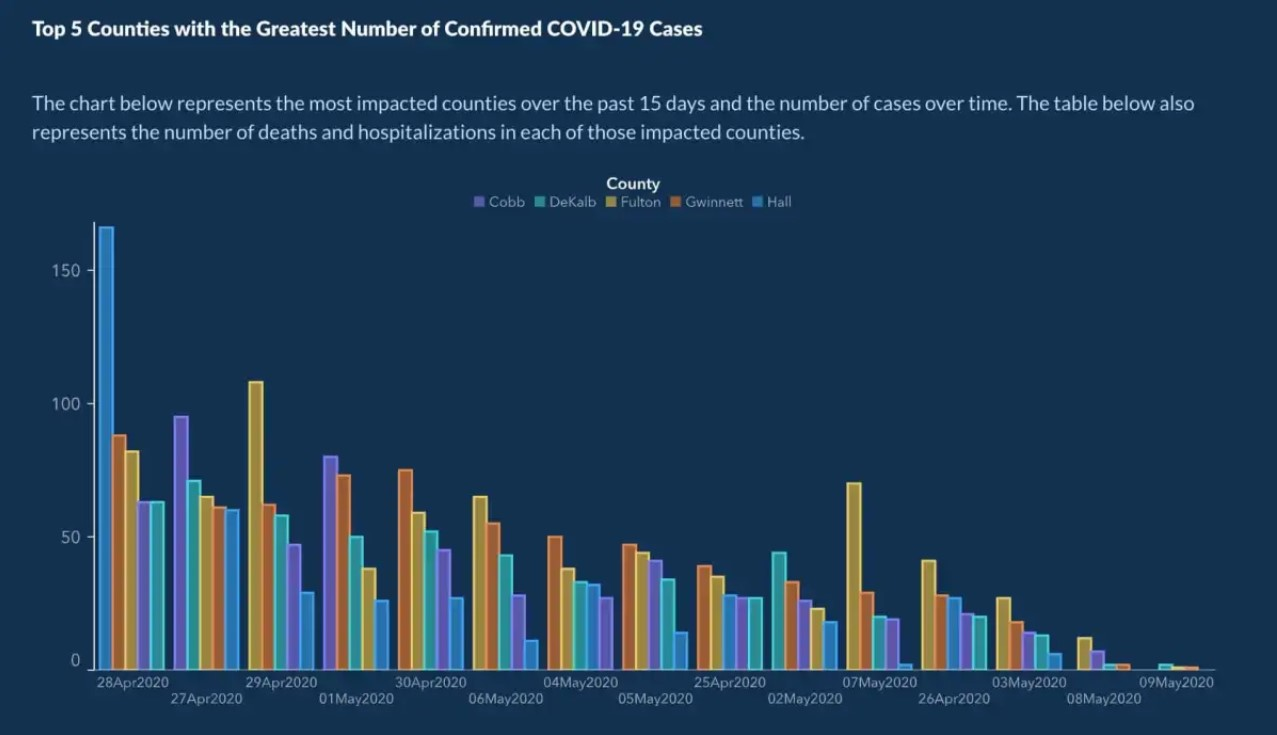
\includegraphics[width=17.74in]{original_graphs/covid19_in_georgia} This
is the corrected graph by the GA DPH posted one week after the
misleading one was published. The original graph listed days
non-chronologically, ultimately to give the appearance that the number
of deaths and hospitalizations in the most affected counties in Georgia
were steadily declining.

The manner of this corrected graph is what we will replicate, but we
will alter it to map countries instead of counties in Georgia.

\hypertarget{the-claim}{%
\subsection{The Claim}\label{the-claim}}

The claim from the article is that a graphic posted on the Georgia
Department of Public Health's website was inaccurately made and did not
effectively display the number of deaths and hospitalizations over time.
It showed cases steadily declining---assuming that dates were listed
chronologically---but they weren't.

The author, Kelley, writes: \textgreater{} ``This is of course insane.
Nobody makes graphs with dates in a non-chronological fashion. It's just
wrong. I was very glad to see they fixed it promptly.''

The article notices that there were declining COVID-19-related deaths
and hospitalizations when the data is displayed chronologically over the
15 days measured, but the real decline is unlike the one shown in the
original graph. While there are other corrections that she would still
make to the second GA DPH graph, she believes that the second tells the
story of COVID-related deaths and hospitalizations much more clearly.

We would like to use the data collected and study a different question:
How does COVID-19 infection rates differ country to country over a time
frame?

\hypertarget{design}{%
\subsection{Design}\label{design}}

The author of the GA DPH graphs chose to use a side-by-side bar graph to
compare the reported COVID-19 cases in counties in Georgia over time.
The author may have chosen this graph because bar charts are effective
for visualizing count variables with categorical variables.

There are three variables displayed in this visualization: the date that
the data was collected, the deaths and hospitalizations each given day,
and different counties in Georgia. The date is on the x-axis, deaths and
hospitalizations are in the y-axis, and counties are mapped by a color
aesthetic.

The count of deaths and hospitalization are measured through position on
a common axis while counties are mapped by color.

Mapping counties by color is an effective choice given that the author
wanted to measure those specific counties. However, the graph easily
becomes overwhelming with five different colors and among many days. A
more effective use of color might be to gray out all counties except
one, which would draw a person's attention to that county and how it
compares to others.

This graph is, overall, ineffective in demonstrating which counties have
the highest death and hospitalization rates in Georgia because the
analysis compares numerous ones with similar counts. There are also no
actual counts to give finality to the claim. Additionally, the graph is
lacking trend lines or trend descriptors that would explain how rates
are are either increasing or declining over time, thus decreasing
usefulness of the date variable.

\hypertarget{the-data}{%
\subsection{The Data}\label{the-data}}

Unfortunately, we were not able to find the original data set for the
Georgia graph. However, we found a supplement data set that has the
information that we need to recreate this particular graph on a global
level instead of a state-wide level.

This dataset that we now plan to use comes from
\href{https://ourworldindata.org/covid-cases}{Our World in Data} and
measures various indicators on COVID-19 rates and affects each day
across countries.

This is an open-source data set, meaning that it is accessible for
everyone to use. On the website's terms and conditions, they state,
``You have permission to use, distribute, and reproduce these in any
medium, provided the source and authors are credited. All the software
and code that we write is open source and made available via GitHub
under the permissive MIT license.''

This data can be traced back to the work of Edouard Mathieu, Hannah
Ritchie, Lucas Rodés-Guirao, Cameron Appel, Daniel Gavrilov, Charlie
Giattino, Joe Hasell, Bobbie Macdonald, Saloni Dattani, Diana Beltekian,
Esteban Ortiz-Ospina, Max Roser, Carl Bergstrom, Bernadeta Dadonaite,
Natalie Dean, Joel Hellewell, Jason Hendry, Adam Kucharski, Moritz
Kraemer and Eric Topol for their very helpful and detailed comments and
suggestions on earlier versions of this work. Also, Tom Chivers is
acknowledged for his editorial review and feedback.

\hypertarget{processing-and-data-collection-process}{%
\subsubsection{Processing and Data Collection
Process:}\label{processing-and-data-collection-process}}

This data relies on Johns Hopkins University. ``The Johns Hopkins
University dashboard and dataset is maintained by a team at its Center
for Systems Science and Engineering (CSSE)\ldots This data is sourced
from governments, national and sub national agencies across the world.''

We believe that this data set was probably made anonymous to an extent
because these are medical records of people's results regarding COVID-19
along with vaccination status. However, the data was also probably
aggregated because it is collected from many different countries and on
many different variables like hospitalizations, deaths, vaccinations.
Another important factor is that it is a compiled summary report for the
purpose of it being public knowledge.

\hypertarget{data-details}{%
\subsubsection{Data Details:}\label{data-details}}

\begin{Shaded}
\begin{Highlighting}[]
\NormalTok{covid\_data }\OtherTok{\textless{}{-}} \FunctionTok{read\_csv}\NormalTok{(}\StringTok{"data/owid{-}covid{-}data.csv"}\NormalTok{)}
\end{Highlighting}
\end{Shaded}

\begin{verbatim}
## Rows: 189999 Columns: 34
## -- Column specification --------------------------------------------------------
## Delimiter: ","
## chr  (5): iso_code, continent, location, date, tests_units
## dbl (29): total_cases, new_cases, new_cases_smoothed, total_deaths, new_deat...
## 
## i Use `spec()` to retrieve the full column specification for this data.
## i Specify the column types or set `show_col_types = FALSE` to quiet this message.
\end{verbatim}

\begin{Shaded}
\begin{Highlighting}[]
\NormalTok{new\_covid\_date }\OtherTok{\textless{}{-}}\NormalTok{ covid\_data }\SpecialCharTok{\%\textgreater{}\%} 
  \FunctionTok{mutate}\NormalTok{(}\AttributeTok{date =}\NormalTok{ lubridate}\SpecialCharTok{::}\FunctionTok{dmy}\NormalTok{(date))}

\FunctionTok{head}\NormalTok{(new\_covid\_date)}
\end{Highlighting}
\end{Shaded}

\begin{verbatim}
## # A tibble: 6 x 34
##   iso_code continent location  date       total_cases new_cases new_cases_smoot~
##   <chr>    <chr>     <chr>     <date>           <dbl>     <dbl>            <dbl>
## 1 AFG      Asia      Afghanis~ 2020-02-24           5         5            0    
## 2 AFG      Asia      Afghanis~ 2020-02-25           5         0            0    
## 3 AFG      Asia      Afghanis~ 2020-02-26           5         0            0    
## 4 AFG      Asia      Afghanis~ 2020-02-27           5         0            0    
## 5 AFG      Asia      Afghanis~ 2020-02-28           5         0            0    
## 6 AFG      Asia      Afghanis~ 2020-02-29           5         0            0.714
## # ... with 27 more variables: total_deaths <dbl>, new_deaths <dbl>,
## #   new_deaths_smoothed <dbl>, total_cases_per_million <dbl>,
## #   new_cases_per_million <dbl>, total_deaths_per_million <dbl>,
## #   reproduction_rate <dbl>, hosp_patients <dbl>, total_tests <dbl>,
## #   positive_rate <dbl>, tests_units <chr>, total_vaccinations <dbl>,
## #   people_vaccinated <dbl>, people_fully_vaccinated <dbl>,
## #   total_boosters <dbl>, new_vaccinations <dbl>, stringency_index <dbl>, ...
\end{verbatim}

Each row represents the status of a country in one day in relation to
the spread and effects of COVID-19. In total, there are 189999
observations that correlate with 34 columns with each observation. Among
those columns are the \texttt{continent}, \texttt{location} (country),
the \texttt{date}, and how many \texttt{new\ cases} there are.
Additionally, the dataset records \texttt{total\ cases},
\texttt{total\ deaths}, \texttt{new\ deaths}, and, information related
to testing, vaccination, country demographics, and rates of health
problems that may affect a person's reaction to the virus.

This data focuses on cases, deaths, and vaccinations by the millions
because global COVID counts are so large.

\hypertarget{wrangling}{%
\subsection{Wrangling}\label{wrangling}}

To replicate the Georgia graph with our world data, we need to only
select the columns \texttt{continent}, \texttt{location}, \texttt{date},
and \texttt{total\_cases}. From there, we would like the continent of
Europe to be like Georgia, and filter for 5 countries that will
represent our Georgia counties.

At a broader level, for each specific continent, we chose 5 different
countries based on population or how popular the country is. Then from
the bigger data frame (new\_covid\_date), we selected continent,
location, date, and how many new cases the country had at specific
dates. From there, we filtered out the countries from the specific
continent that we wanted and created the new dataset for each of the
continents.

The bigger data frame (new\_covid\_date) had to be adjusted because of
the date type that was originally set in the data. If we had not mutated
the data type, it was very hard to pull the specific dates that we
wanted for the graphs. Therefore, that needed to be changed.

\begin{Shaded}
\begin{Highlighting}[]
\NormalTok{location\_list }\OtherTok{\textless{}{-}} \FunctionTok{list}\NormalTok{(}\StringTok{"France"}\NormalTok{, }\StringTok{"Germany"}\NormalTok{, }\StringTok{"Italy"}\NormalTok{, }\StringTok{"Russia"}\NormalTok{, }\StringTok{"Poland"}\NormalTok{)}

\NormalTok{europe }\OtherTok{\textless{}{-}}\NormalTok{ new\_covid\_date }\SpecialCharTok{\%\textgreater{}\%} 
  \FunctionTok{select}\NormalTok{(continent, location, date, new\_cases) }\SpecialCharTok{\%\textgreater{}\%} 
  \FunctionTok{filter}\NormalTok{(continent }\SpecialCharTok{==} \StringTok{"Europe"}\NormalTok{) }\SpecialCharTok{\%\textgreater{}\%} 
  \FunctionTok{filter}\NormalTok{(location }\SpecialCharTok{\%in\%}\NormalTok{ location\_list)}
\end{Highlighting}
\end{Shaded}

This code chunk is set specific to Europe. The location\_list contains
all of the countries we are focusing on. From there, we selected the
continent, location, date, and how many new\_cases. Then filtered out
specifically what we were looking for.

\begin{Shaded}
\begin{Highlighting}[]
\NormalTok{aslocation\_list }\OtherTok{\textless{}{-}} \FunctionTok{list}\NormalTok{(}\StringTok{"China"}\NormalTok{, }\StringTok{"India"}\NormalTok{, }\StringTok{"Indonesia"}\NormalTok{, }\StringTok{"Pakistan"}\NormalTok{, }\StringTok{"Bangladesh"}\NormalTok{)}

\NormalTok{asia }\OtherTok{\textless{}{-}}\NormalTok{ new\_covid\_date }\SpecialCharTok{\%\textgreater{}\%} 
  \FunctionTok{select}\NormalTok{(continent, location, date, new\_cases) }\SpecialCharTok{\%\textgreater{}\%} 
  \FunctionTok{filter}\NormalTok{(continent }\SpecialCharTok{==} \StringTok{"Asia"}\NormalTok{) }\SpecialCharTok{\%\textgreater{}\%} 
  \FunctionTok{filter}\NormalTok{(location }\SpecialCharTok{\%in\%}\NormalTok{ aslocation\_list)}
\end{Highlighting}
\end{Shaded}

This code chunk is set specific to Asia. The aslocation\_list contains
all of the countries we are focusing on. From there, we selected the
continent, location, date, and how many new\_cases. Then filtered out
specifically what we were looking for.

\begin{Shaded}
\begin{Highlighting}[]
\NormalTok{aflocation\_list }\OtherTok{\textless{}{-}} \FunctionTok{list}\NormalTok{(}\StringTok{"Algeria"}\NormalTok{, }\StringTok{"Egypt"}\NormalTok{, }\StringTok{"Libya"}\NormalTok{, }\StringTok{"Ethiopia"}\NormalTok{, }\StringTok{"Nigeria"}\NormalTok{)}

\NormalTok{africa }\OtherTok{\textless{}{-}}\NormalTok{ new\_covid\_date }\SpecialCharTok{\%\textgreater{}\%} 
  \FunctionTok{select}\NormalTok{(continent, location, date, new\_cases) }\SpecialCharTok{\%\textgreater{}\%} 
  \FunctionTok{filter}\NormalTok{(continent }\SpecialCharTok{==} \StringTok{"Africa"}\NormalTok{) }\SpecialCharTok{\%\textgreater{}\%} 
  \FunctionTok{filter}\NormalTok{(location }\SpecialCharTok{\%in\%}\NormalTok{ aflocation\_list)}
\end{Highlighting}
\end{Shaded}

This code chunk is set specific to Africa. The aflocation\_list contains
all of the countries we are focusing on. From there, we selected the
continent, location, date, and how many new\_cases. Then filtered out
specifically what we were looking for.

\begin{Shaded}
\begin{Highlighting}[]
\NormalTok{salocation\_list }\OtherTok{\textless{}{-}} \FunctionTok{list}\NormalTok{(}\StringTok{"Brazil"}\NormalTok{, }\StringTok{"Colombia"}\NormalTok{, }\StringTok{"Argentina"}\NormalTok{, }\StringTok{"Peru"}\NormalTok{, }\StringTok{"Chile"}\NormalTok{)}

\NormalTok{southamerica }\OtherTok{\textless{}{-}}\NormalTok{ new\_covid\_date }\SpecialCharTok{\%\textgreater{}\%} 
  \FunctionTok{select}\NormalTok{(continent, location, date, new\_cases) }\SpecialCharTok{\%\textgreater{}\%} 
  \FunctionTok{filter}\NormalTok{(continent }\SpecialCharTok{==} \StringTok{"South America"}\NormalTok{) }\SpecialCharTok{\%\textgreater{}\%} 
  \FunctionTok{filter}\NormalTok{(location }\SpecialCharTok{\%in\%}\NormalTok{ salocation\_list)}
\end{Highlighting}
\end{Shaded}

This code chunk is set specific to South America. The salocation\_list
contains all of the countries we are focusing on. From there, we
selected the continent, location, date, and how many new\_cases. Then
filtered out specifically what we were looking for.

\begin{Shaded}
\begin{Highlighting}[]
\NormalTok{olocation\_list }\OtherTok{\textless{}{-}} \FunctionTok{list}\NormalTok{(}\StringTok{"Papua New Guinea"}\NormalTok{, }\StringTok{"New Zealand"}\NormalTok{, }\StringTok{"Fiji"}\NormalTok{, }\StringTok{"Solomon Islands"}\NormalTok{, }\StringTok{"French Polynesia"}\NormalTok{)}

\NormalTok{oceania }\OtherTok{\textless{}{-}}\NormalTok{ new\_covid\_date }\SpecialCharTok{\%\textgreater{}\%} 
  \FunctionTok{select}\NormalTok{(continent, location, date, total\_cases, total\_tests, total\_vaccinations,total\_deaths, new\_cases) }\SpecialCharTok{\%\textgreater{}\%} 
  \FunctionTok{filter}\NormalTok{(continent }\SpecialCharTok{==} \StringTok{"Oceania"}\NormalTok{) }\SpecialCharTok{\%\textgreater{}\%} 
  \FunctionTok{filter}\NormalTok{(location }\SpecialCharTok{\%in\%}\NormalTok{ olocation\_list)}
\end{Highlighting}
\end{Shaded}

This code chunk is set specific to Oceania. The olocation\_list contains
all of the countries we are focusing on. From there, we selected the
continent, location, date, and how many new\_cases. Then filtered out
specifically what we were looking for.

\begin{Shaded}
\begin{Highlighting}[]
\NormalTok{africa}\SpecialCharTok{|\textgreater{}}
  \FunctionTok{filter}\NormalTok{(}\FunctionTok{between}\NormalTok{(date,}\FunctionTok{as.Date}\NormalTok{(}\StringTok{\textquotesingle{}2021{-}04{-}28\textquotesingle{}}\NormalTok{), }\FunctionTok{as.Date}\NormalTok{(}\StringTok{\textquotesingle{}2021{-}05{-}09\textquotesingle{}}\NormalTok{))) }\SpecialCharTok{|\textgreater{}}
  \FunctionTok{ggplot}\NormalTok{() }\SpecialCharTok{+}
  \CommentTok{\#coord\_flip() +}
  \FunctionTok{aes}\NormalTok{(}\AttributeTok{x =}\NormalTok{ date, }\AttributeTok{y =}\NormalTok{ new\_cases, }\AttributeTok{fill =}\NormalTok{ location) }\SpecialCharTok{+}
  \FunctionTok{geom\_col}\NormalTok{(}\AttributeTok{position =} \StringTok{"dodge"}\NormalTok{) }\SpecialCharTok{+}
  \FunctionTok{scale\_fill\_viridis\_d}\NormalTok{() }\SpecialCharTok{+}
  \FunctionTok{scale\_fill\_brewer}\NormalTok{(}\AttributeTok{palette =} \StringTok{"GnBu"}\NormalTok{) }\SpecialCharTok{+}
  \FunctionTok{theme\_dark}\NormalTok{() }\SpecialCharTok{+}
  \FunctionTok{theme}\NormalTok{(}\AttributeTok{legend.position=}\StringTok{"top"}\NormalTok{) }\SpecialCharTok{+}
   \FunctionTok{labs}\NormalTok{(}\AttributeTok{x=}\StringTok{"Dates from April 28th {-} May 9th }\SpecialCharTok{\textbackslash{}n}\StringTok{ 2021"}\NormalTok{,}
       \AttributeTok{y =} \StringTok{"Total New Cases"}\NormalTok{,}
       \AttributeTok{fill =} \StringTok{"Locations"}\NormalTok{,}
       \AttributeTok{title =} \StringTok{"Daily New Cases from selected countries in Africa"}\NormalTok{,}
       \AttributeTok{subtitle =} \StringTok{"Algeria, Egypt, Nigeria, Ethiopia, Libya"}\NormalTok{ ,}
       \AttributeTok{caption =} \StringTok{"Source: OWID"}\NormalTok{)}
\end{Highlighting}
\end{Shaded}

\begin{verbatim}
## Scale for 'fill' is already present. Adding another scale for 'fill', which
## will replace the existing scale.
\end{verbatim}

\includegraphics{milestone2_files/figure-latex/replicated graph: Africa-1.pdf}

\begin{Shaded}
\begin{Highlighting}[]
\NormalTok{asia}\SpecialCharTok{|\textgreater{}}
  \FunctionTok{filter}\NormalTok{(}\FunctionTok{between}\NormalTok{(date,}\FunctionTok{as.Date}\NormalTok{(}\StringTok{\textquotesingle{}2020{-}04{-}28\textquotesingle{}}\NormalTok{), }\FunctionTok{as.Date}\NormalTok{(}\StringTok{\textquotesingle{}2020{-}05{-}09\textquotesingle{}}\NormalTok{))) }\SpecialCharTok{|\textgreater{}}
  \FunctionTok{ggplot}\NormalTok{() }\SpecialCharTok{+}
  \CommentTok{\#coord\_flip() +}
  \FunctionTok{aes}\NormalTok{(}\AttributeTok{x =}\NormalTok{ date, }\AttributeTok{y =}\NormalTok{ new\_cases, }\AttributeTok{fill =}\NormalTok{ location) }\SpecialCharTok{+}
  \FunctionTok{geom\_col}\NormalTok{(}\AttributeTok{position =} \StringTok{"dodge"}\NormalTok{) }\SpecialCharTok{+}
  \FunctionTok{scale\_fill\_viridis\_d}\NormalTok{() }\SpecialCharTok{+}
  \FunctionTok{scale\_fill\_brewer}\NormalTok{(}\AttributeTok{palette =} \StringTok{"PuRd"}\NormalTok{) }\SpecialCharTok{+}
  \FunctionTok{theme\_dark}\NormalTok{() }\SpecialCharTok{+}
  \FunctionTok{theme}\NormalTok{(}\AttributeTok{legend.position=}\StringTok{"top"}\NormalTok{) }\SpecialCharTok{+}
  \FunctionTok{labs}\NormalTok{(}\AttributeTok{x=}\StringTok{"Dates from April 28th {-} May 9th }\SpecialCharTok{\textbackslash{}n}\StringTok{ 2021"}\NormalTok{,}
       \AttributeTok{y =} \StringTok{"Total New Cases"}\NormalTok{,}
       \AttributeTok{fill =} \StringTok{"Locations"}\NormalTok{,}
       \AttributeTok{title =} \StringTok{"Daily New Cases from selected countries in Asia"}\NormalTok{,}
       \AttributeTok{subtitle =} \StringTok{"Bangladesh, China, India, Indonesia, Pakistan"}\NormalTok{,}
       \AttributeTok{caption =} \StringTok{"Source: OWID"}\NormalTok{)}
\end{Highlighting}
\end{Shaded}

\begin{verbatim}
## Scale for 'fill' is already present. Adding another scale for 'fill', which
## will replace the existing scale.
\end{verbatim}

\includegraphics{milestone2_files/figure-latex/replicated graph: Asia-1.pdf}

\begin{Shaded}
\begin{Highlighting}[]
\NormalTok{oceania }\SpecialCharTok{|\textgreater{}}
  \FunctionTok{filter}\NormalTok{(}\FunctionTok{between}\NormalTok{(date,}\FunctionTok{as.Date}\NormalTok{(}\StringTok{\textquotesingle{}2021{-}01{-}20\textquotesingle{}}\NormalTok{), }\FunctionTok{as.Date}\NormalTok{(}\StringTok{\textquotesingle{}2021{-}01{-}25\textquotesingle{}}\NormalTok{))) }\SpecialCharTok{|\textgreater{}}
  \FunctionTok{ggplot}\NormalTok{() }\SpecialCharTok{+}
  \CommentTok{\#coord\_flip() +}
  \FunctionTok{aes}\NormalTok{(}\AttributeTok{x =}\NormalTok{ date, }\AttributeTok{y =}\NormalTok{ new\_cases, }\AttributeTok{fill =}\NormalTok{ location) }\SpecialCharTok{+}
  \FunctionTok{geom\_col}\NormalTok{(}\AttributeTok{position =} \StringTok{"dodge"}\NormalTok{) }\SpecialCharTok{+}
  \FunctionTok{scale\_fill\_viridis\_d}\NormalTok{() }\SpecialCharTok{+}
  \FunctionTok{scale\_fill\_brewer}\NormalTok{(}\AttributeTok{palette =} \StringTok{"OrRd"}\NormalTok{) }\SpecialCharTok{+}
  \FunctionTok{theme\_dark}\NormalTok{() }\SpecialCharTok{+}
  \FunctionTok{theme}\NormalTok{(}\AttributeTok{legend.position=}\StringTok{"top"}\NormalTok{) }\SpecialCharTok{+}
   \FunctionTok{labs}\NormalTok{(}\AttributeTok{x=}\StringTok{"Dates from Janurary 20th{-}25th }\SpecialCharTok{\textbackslash{}n}\StringTok{ 2020"}\NormalTok{,}
       \AttributeTok{y =} \StringTok{"Total New Cases"}\NormalTok{,}
       \AttributeTok{fill =} \StringTok{"Locations"}\NormalTok{,}
       \AttributeTok{title =} \StringTok{"Daily New Cases from selected countries in Oceania"}\NormalTok{,}
       \AttributeTok{subtitle =} \StringTok{"Papua New Guinea, New Zealand, Fiji, Solomon Islands, French Polynesia"}\NormalTok{ ,}
       \AttributeTok{caption =} \StringTok{"Source: OWID"}\NormalTok{)}
\end{Highlighting}
\end{Shaded}

\begin{verbatim}
## Scale for 'fill' is already present. Adding another scale for 'fill', which
## will replace the existing scale.
\end{verbatim}

\includegraphics{milestone2_files/figure-latex/replicated graph: Oceania-1.pdf}

\begin{Shaded}
\begin{Highlighting}[]
\NormalTok{southamerica}\SpecialCharTok{|\textgreater{}}
  \FunctionTok{filter}\NormalTok{(}\FunctionTok{between}\NormalTok{(date,}\FunctionTok{as.Date}\NormalTok{(}\StringTok{\textquotesingle{}2022{-}01{-}20\textquotesingle{}}\NormalTok{), }\FunctionTok{as.Date}\NormalTok{(}\StringTok{\textquotesingle{}2022{-}01{-}25\textquotesingle{}}\NormalTok{))) }\SpecialCharTok{|\textgreater{}}
  \FunctionTok{ggplot}\NormalTok{() }\SpecialCharTok{+}
  \CommentTok{\#coord\_flip() +}
  \FunctionTok{aes}\NormalTok{(}\AttributeTok{x =}\NormalTok{ date, }\AttributeTok{y =}\NormalTok{ new\_cases, }\AttributeTok{fill =}\NormalTok{ location) }\SpecialCharTok{+}
  \FunctionTok{geom\_col}\NormalTok{(}\AttributeTok{position =} \StringTok{"dodge"}\NormalTok{) }\SpecialCharTok{+}
  \FunctionTok{scale\_fill\_viridis\_d}\NormalTok{() }\SpecialCharTok{+}
  \FunctionTok{scale\_fill\_brewer}\NormalTok{(}\AttributeTok{palette =} \StringTok{"YlGn"}\NormalTok{) }\SpecialCharTok{+}
  \FunctionTok{theme\_dark}\NormalTok{() }\SpecialCharTok{+}
  \FunctionTok{theme}\NormalTok{(}\AttributeTok{legend.position=}\StringTok{"top"}\NormalTok{) }\SpecialCharTok{+}
   \FunctionTok{labs}\NormalTok{(}\AttributeTok{x=}\StringTok{"Dates from Janurary 20th{-}25th }\SpecialCharTok{\textbackslash{}n}\StringTok{ 2022"}\NormalTok{,}
       \AttributeTok{y =} \StringTok{"Total New Cases"}\NormalTok{,}
       \AttributeTok{fill =} \StringTok{"Locations"}\NormalTok{,}
       \AttributeTok{title =} \StringTok{"Daily New Cases from selected countries in South America"}\NormalTok{,}
       \AttributeTok{subtitle =} \StringTok{"Peru, Colombia, Chile, Brazil, Argentina "}\NormalTok{ ,}
       \AttributeTok{caption =} \StringTok{"Source: OWID"}\NormalTok{)}
\end{Highlighting}
\end{Shaded}

\begin{verbatim}
## Scale for 'fill' is already present. Adding another scale for 'fill', which
## will replace the existing scale.
\end{verbatim}

\includegraphics{milestone2_files/figure-latex/replicated graph: South America-1.pdf}

\begin{Shaded}
\begin{Highlighting}[]
\NormalTok{europe}\SpecialCharTok{|\textgreater{}}
  \FunctionTok{filter}\NormalTok{(}\FunctionTok{between}\NormalTok{(date,}\FunctionTok{as.Date}\NormalTok{(}\StringTok{\textquotesingle{}2020{-}09{-}20\textquotesingle{}}\NormalTok{), }\FunctionTok{as.Date}\NormalTok{(}\StringTok{\textquotesingle{}2020{-}09{-}25\textquotesingle{}}\NormalTok{))) }\SpecialCharTok{|\textgreater{}}
  \FunctionTok{ggplot}\NormalTok{() }\SpecialCharTok{+}
  \CommentTok{\#coord\_flip() +}
  \FunctionTok{aes}\NormalTok{(}\AttributeTok{x =}\NormalTok{ date, }\AttributeTok{y =}\NormalTok{ new\_cases, }\AttributeTok{fill =}\NormalTok{ location) }\SpecialCharTok{+}
  \FunctionTok{geom\_col}\NormalTok{(}\AttributeTok{position =} \StringTok{"dodge"}\NormalTok{) }\SpecialCharTok{+}
  \FunctionTok{scale\_fill\_viridis\_d}\NormalTok{() }\SpecialCharTok{+}
  \FunctionTok{scale\_fill\_brewer}\NormalTok{(}\AttributeTok{palette =} \StringTok{"PuBuGn"}\NormalTok{) }\SpecialCharTok{+}
  \FunctionTok{theme\_dark}\NormalTok{() }\SpecialCharTok{+}
  \FunctionTok{theme}\NormalTok{(}\AttributeTok{legend.position=}\StringTok{"top"}\NormalTok{) }\SpecialCharTok{+}
   \FunctionTok{labs}\NormalTok{(}\AttributeTok{x=}\StringTok{"Dates from Sept 20th{-}25th }\SpecialCharTok{\textbackslash{}n}\StringTok{ 2021"}\NormalTok{,}
       \AttributeTok{y =} \StringTok{"Total New Cases"}\NormalTok{,}
       \AttributeTok{fill =} \StringTok{"Locations"}\NormalTok{,}
       \AttributeTok{title =} \StringTok{"Daily New Cases from selected countries in Europe"}\NormalTok{,}
       \AttributeTok{subtitle =} \StringTok{"France, Germany, Italy, Poland, Russia"}\NormalTok{ ,}\AttributeTok{caption =} \StringTok{"Source: OWID"}\NormalTok{)}
\end{Highlighting}
\end{Shaded}

\begin{verbatim}
## Scale for 'fill' is already present. Adding another scale for 'fill', which
## will replace the existing scale.
\end{verbatim}

\includegraphics{milestone2_files/figure-latex/replicated graph: Europe-1.pdf}

\hypertarget{replication}{%
\subsection{Replication}\label{replication}}

The code above is our steps to replicating the graph from article 1. One
of the difficulties we encountered was first trying to pull dates from
the specific continent data frame. It took a while until we asked the
professor how. The basics of constructing a bar graph were all the same.
When comparing a lab to the replication, we had to depend on ourselves
for everything. Time consumption was another difficulty because we
wanted to replicate five different graphs for one.

\hypertarget{alternative-graph-1}{%
\subsection{Alternative Graph \#1}\label{alternative-graph-1}}

One alternative graph for our data comes from
\href{https://ourworldindata.org/grapher/daily-cases-covid-region?time=2022-01-01..2022-09-30}{Our
World in Data}. The site allows a viewer to interact with the graph by
customizing the variables mapped and the scale of time on the x-axis.
Through this customization, we created the graph below.

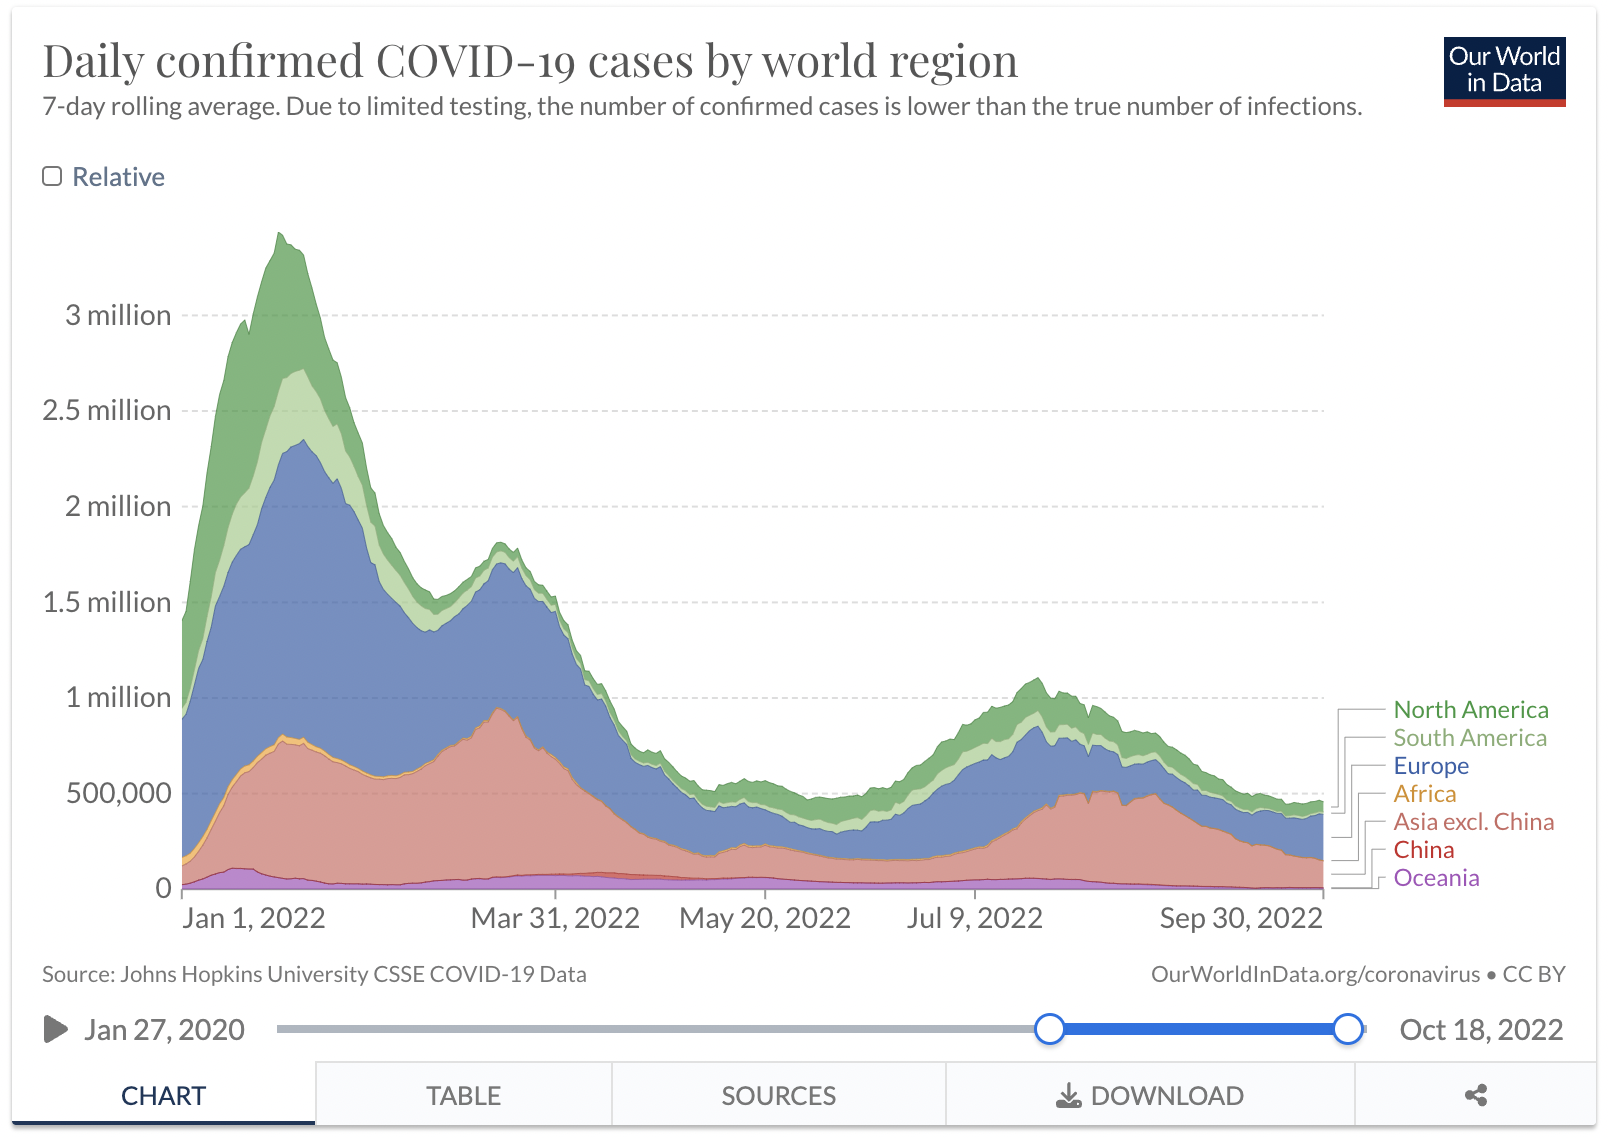
\includegraphics[width=22.33in]{original_graphs/our_world_in_data_graphic}
\#\#\# Alternative \#1: Design

This data from Our World in Data is presented here through a stacked
density graph to visualize the total number of new COVID-19 cases and
overall trends that are occurring while allowing the viewer to also note
case differences among different continents.

The date from January 1, 2022 to September 30, 2022 is being measured on
the x-axis while daily confirmed cases is on the y-axis and continents
are mapped by color. Position on a common scale is they key for
comparison over time.

For this graph, color is an effective way to map continents because
there are only 7 continents that need to be registered. The smooth flow
of case numbers helps color transitions to be easy on the eyes while
still allowing us to see which continents seem to be hit hardest.
Because this graph is interactive on the website, there is an option to
hover over a colored portion of the graph and only see that continent in
color while the others are grayed out. This is an especially effective
use of the color aesthetic.

Visualizing overall trends is one of the strengths of this graph. We can
see worldly trends while also understanding which continents seem to be
most heavily affected. However, this graph makes comparing continents
with each other and seeing their trends especially challenging since
densities of count in continents are stacked on top of each other.
Additionally, this graph doesn't factor in continent populations, which
is one of the biggest predictors of COVID-19 cases, thereby leaving out
a significant factor of COVID's story.

The biggest choice in this graph compared to the prior is that cases are
visualized on a worldly scale instead of segmented. It shows that,
despite distance, the world is going through the same pandemic.

The claim in the original graph is that affects of COVID are
fluctuating, so COVID protections should not end here. The waves of
density in this graph also show the fluctuation and suggest that COVID
is too unpredictable to relax, but the claim that cases are declining is
also perpetuated. Ultimately, they have a similar claim.

\hypertarget{alternative-1-implementation}{%
\subsubsection{Alternative \#1:
Implementation}\label{alternative-1-implementation}}

We really appreciate the density structure of the alternative design,
but we disliked how the stacked aspect of it made it hard to directly
compare COVID case rates in countries. Therefore, in the implementation
of our alternative, we used a similar structure but faceted the graph by
different countries.

\begin{Shaded}
\begin{Highlighting}[]
\NormalTok{europe}\SpecialCharTok{|\textgreater{}}
  \FunctionTok{filter}\NormalTok{(}\FunctionTok{between}\NormalTok{(date,}\FunctionTok{as.Date}\NormalTok{(}\StringTok{\textquotesingle{}2021{-}06{-}02\textquotesingle{}}\NormalTok{), }\FunctionTok{as.Date}\NormalTok{(}\StringTok{\textquotesingle{}2021{-}07{-}09\textquotesingle{}}\NormalTok{))) }\SpecialCharTok{|\textgreater{}}
  \FunctionTok{ggplot}\NormalTok{() }\SpecialCharTok{+}
  \CommentTok{\#coord\_flip() +}
  \FunctionTok{aes}\NormalTok{(}\AttributeTok{x =}\NormalTok{ date, }\AttributeTok{y =}\NormalTok{ new\_cases, }\AttributeTok{fill =}\NormalTok{ location) }\SpecialCharTok{+}
  \FunctionTok{facet\_wrap}\NormalTok{(}\SpecialCharTok{\textasciitilde{}}\NormalTok{location, }\AttributeTok{scales =} \StringTok{"free\_y"}\NormalTok{) }\SpecialCharTok{+}
  \FunctionTok{geom\_area}\NormalTok{(}\AttributeTok{color=}\StringTok{"darkred"}\NormalTok{) }\SpecialCharTok{+}
  \FunctionTok{scale\_fill\_viridis\_d}\NormalTok{() }\SpecialCharTok{+}
  \CommentTok{\#scale\_fill\_brewer(palette = "GnBu") +}
  \FunctionTok{theme\_dark}\NormalTok{() }\SpecialCharTok{+}
  \FunctionTok{theme}\NormalTok{(}\AttributeTok{legend.position=}\StringTok{"top"}\NormalTok{) }\SpecialCharTok{+}
   \FunctionTok{labs}\NormalTok{(}\AttributeTok{x=}\StringTok{"Dates from June 2th {-} July 9th }\SpecialCharTok{\textbackslash{}n}\StringTok{ 2021"}\NormalTok{,}
       \AttributeTok{y =} \StringTok{"Total New Cases"}\NormalTok{,}
       \AttributeTok{fill =} \StringTok{"Locations"}\NormalTok{,}
       \AttributeTok{title =} \StringTok{"Daily New Cases from selected countries in Europe"}\NormalTok{,}
       \AttributeTok{subtitle =} \StringTok{"France, Germany, Italy, Poland, Russia"}\NormalTok{ ,}
       \AttributeTok{caption =} \StringTok{"Source: OWID"}\NormalTok{)}
\end{Highlighting}
\end{Shaded}

\includegraphics{milestone2_files/figure-latex/alternative data graph: Europe-1.pdf}
\#\# Alternative Graph \#2

Our next alternative graph that we found and admire comes from a Twitter
page called \href{https://mobile.twitter.com/covid19tracking}{The COVID
Tracking Project}, which completes analyses on COVID-19 and gives
regular updates to the public.

\begin{quote}
``The COVID Tracking Project collects and publishes the most complete
testing data available for US states and territories.''
\end{quote}

The graph that we would like to highlight from their page is a faceted
histogram with a kernel density estimation line over it to show how the
average number of tests in 7 days, the average number of cases in 7
days, the average current hospitalizations in 7 days, and the average
daily deaths due to COVID-19 in 7 days are fluctuating over 11 months in
the United States.

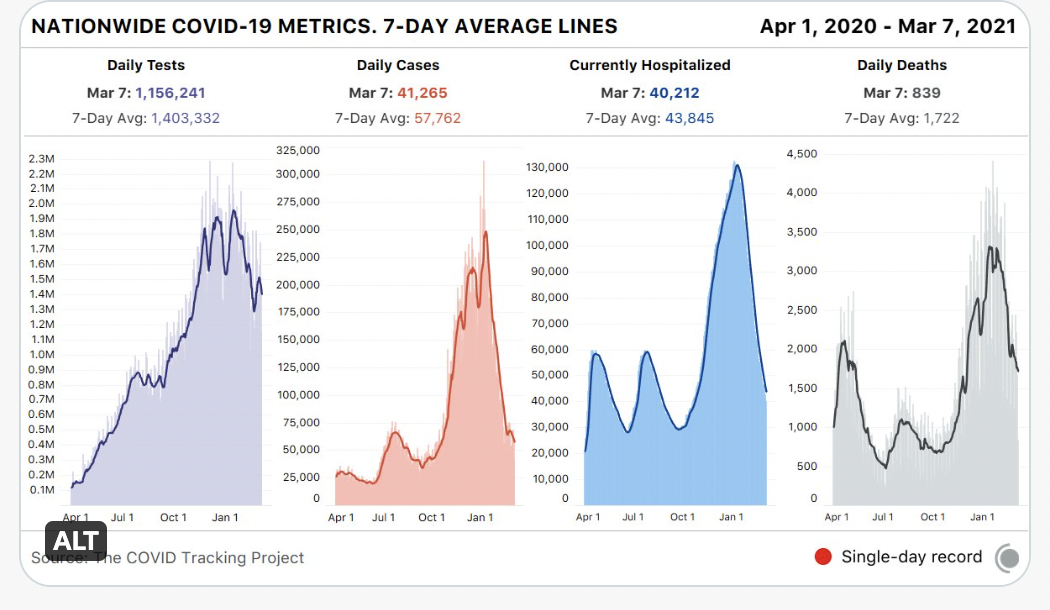
\includegraphics[width=14.58in]{original_graphs/7_day_covid_metrics}
This graph is a faceted histogram with a kernel density estimation lined
over it so that the viewer can easily see trends in COVID-19 metrics
over the 11 months studied. With this faceted graph, the viewer can
compare the overall structure of trend lines among metrics at given
times in the year without looking at a single, overly-crowded plot. This
is especially helpful for measuring different metrics at waves in the
pandemic. We're not quite sure why the author chose to use both
histogram bins and a density trend line, but it does remind the viewer
that weekly averages do not always smoothly transition to the
next---there will likely be sharp increases or decreases depending on
the week's events.

For this graph, time from April 1, 2020 to March 7, 2021 is placed on
the x-axis, and count is on the y-axis. From there, different metrics
are faceted so that their structures can be compared with another. To
make the different plots even easier to differentiate, the author mapped
metrics to different colors.

We think that faceting the graph was an effective choice for protecting
the clarity of the data. Without the facets, it would be hard to see
which color represents each metric, and a viewer would constantly need
to check to see which metric is each color. Because of the facets, the
mapping the color aesthetic to metrics is redundant, but it makes the
graph more visually appealing and signals to the audience that the
faceted graphs are representing different measurements.

Something that we appreciate most about this graph are the numerous
measurements that can be shown and compared to one another. However,
this graph only allows us to view metrics in one country: the United
States. Another con of this graph is that the scale on the y-axis is
different for each metric. While trends are easy to compare, the actual
count data is not.

One of the biggest choices in making this graph was weather or not to
show the y-axes on a fixed scale to accurately reflect counts. The
author decided, instead, to use a continuous scale on each facet, which
we think was a good choice because it allows the wave patterns to be
compared instead of simply the counts, which can be found on any
modeling table. Moreover, it would be impractical to have daily tests,
measured in millions, on the same scale as daily deaths, which are are
measured in thousands.

This change to have a continuous scale for faceted data allows a viewer
to more easily see the fluctuations of COVID and its effects over time,
ultimately showing that we'll never know when the next peak will be. It
also supports the claim that COVID cases are declining.

\hypertarget{summary}{%
\section{Summary}\label{summary}}

🚧 Now that you've gone through the whole process, how has your
understanding of, and belief in, the original article's claim changed?
🚧 How faithful was your replication? 🚧 Compare your original and
alternative designs. Which is best for what purpose? 🚧 What follow-up
questions and ideas do you have about the data or visualization you
worked with? 🚧 How do you feel about this whole experience?

\hypertarget{acknowledgements}{%
\section{Acknowledgements:}\label{acknowledgements}}

\hypertarget{from-abby-ham}{%
\subsubsection{From Abby Ham:}\label{from-abby-ham}}

Abby gave us many great suggestions, one of them being that, as we
analyze the first graph from the COVID-19 in Georgia article, we should
further explain the errors in the Georgia Department of Public Health's
original graph and include that in our document. Then we should explain
what graphic choices the author made in their replication and why we
believe it's fitting for the data.

Secondly, she recommended that we clarify what we are measuring on the
y-axis of each graph (total new cases, total deaths, etc.) and explain
why we made this choice.

Finally, she suggested that we go into greater detail in explaining why
we are using world COVID data instead of the original data because it
was a little confusing how we made that switch.

\hypertarget{from-felicia-and-suha}{%
\subsubsection{From Felicia and Suha:}\label{from-felicia-and-suha}}

One of the first things that they noticed while looking at our file is
how overwhelming portions of it look. Instead of using glimpse() or
summary() to give general ideas on what datasets look like, they
suggested to use head(). This will display headings and the first few
rows of our data without overcrowding the page.

For their project, they keep sections organized by using different
formatting in places. Specifically, they use \textgreater{} in
formatting the claims of articles. This helps differentiate between
their words and the words and thoughts of author data scientists. They
recommended that we also give this a try.

Finally, they noticed that some of our heading sizes and when we insert
headings is inconsistent across sections of our report. They suggested
that we keep headings consistent and use them more intentionally.

\end{document}
